\documentclass[a4paper]{article}
\usepackage{ctex}
\usepackage[affil-it]{authblk}
\usepackage[backend=bibtex,style=numeric]{biblatex}
\usepackage{amsmath,amsthm,amssymb,amsfonts}
\usepackage{graphicx}
\usepackage{bm}

\usepackage{geometry}
\geometry{margin=1.5cm, vmargin={0pt,1cm}}
\setlength{\topmargin}{-1cm}
\setlength{\paperheight}{29.7cm}
\setlength{\textheight}{25.3cm}

\addbibresource{citation.bib}

\begin{document}
% =================================================
\title{微分方程数值解 2026 春夏作业五}

\author{曾申昊 3220100701
  \thanks{邮箱: \texttt{3097714673@qq.com}
                            \texttt{或} \texttt{3220100701@zju.edu.cn}}}
\affil{浙江大学}

\date{更新时间: \today}

\maketitle

% ============================================
\section*{Exercise 13.5}

\par 对于改进 Euler 方法，其迭代公式为
\begin{equation}
    \left\{
        \begin{aligned}
            &y_1 = f(U^n,t_n) \\
            &y_2 = f\Big(U^n+ky_1,t_{n+1}\Big) \\
            &U^{n+1} = U^n + \frac{k}{2}(y_1+y_2) \\
        \end{aligned}
    \right.
\end{equation}
\par 先对 $y_2$ 进行 Taylor 展开
\begin{equation}
    \begin{aligned}
        y_2 &= f\Big(U^n+kf(U^n,t_n),t_{n+1}\Big) \\
        &= f 
        + \left(kf_t + kf f_u\right)
        + \left(
            \frac{k^2}{2} f_{tt} + k^2f f_{ut} + \frac{(kf)^2}{2}  f_{uu}
        \right) + O(k^3)
    \end{aligned}
\end{equation} 
\par 其一步误差为
\begin{equation}
    \begin{aligned}
        \mathcal{L}u(t_n)
        =&\ u(t_{n+1}) - u(t_n) - \frac{k}{2}\left(
            y_1+y_2
        \right) \\
        =&\ \left[
            u(t_n) +ku'(t_n)+\frac{k^2}{2}u''(t_n)+\frac{k^3}{6}u'''(t_n) - u(t_n) + O(k^4)
        \right]  \\
        &- \frac{k}{2}\left[
            f+f 
        + \left(kf_t + kf f_u\right)
        + \left(
            \frac{k^2}{2} f_{tt} + k^2f f_{ut} + \frac{(kf)^2}{2}  f_{uu}
        \right) + O(k^3)
        \right]\\
        =&\ \left[
            kf+\frac{k^2}{2}\left(ff_u+f_t\right)+\frac{k^3}{6}\left(
                f^2_uf+f_uf_t+f^2f_{uu}+2ff_{ut}+f_{tt}
            \right) + O(k^4)
        \right]  \\
        &- \frac{k}{2}\left[
            2f
        + \left(kf_t + kf f_u\right)
        + \left(
            \frac{k^2}{2} f_{tt} + k^2f f_{ut} + \frac{(kf)^2}{2}  f_{uu}
        \right) + O(k^3)
        \right]\\
        =&\ \frac{1}{12}k^3\left(
            2f^2_uf+2f_uf_t-f^2f_{uu}-2ff_{ut}-f_{tt}
        \right) + O(k^4)
    \end{aligned}
\end{equation}
\par 另一边，对于 \textbf{Definition 13.3} 中图像，
粗实线的长度为
\begin{equation}
    \begin{aligned}
        \text{Len} & = u(t_{n+1}) - U^{n+1}\\
        &= u(t_{n+1}) - U^n - \frac{k}{2}\left[
            f(U^n,t_n)+f\Big(U^n+kf(U^n,t_n),t_{n+1}\Big)
        \right] \\
    \end{aligned}
\end{equation}
\par 若 $U^n=u(t_n)$ 则上面两个式子相等。
对于显式中点方法同理可得
\begin{equation}
    \begin{aligned}
        \text{Len} & = u(t_{n+1}) - U^{n+1}\\
        &= u(t_{n+1}) - U^n - k
            f\left(U^n+\frac{k}{2}f(U^n,t_n),t_{n}+\frac{k}{2}\right)
        \\
    \end{aligned}
\end{equation}

\section*{Exercise 13.7}

\par 如图 \ref{fig:Exercise13-7} 所示，
其中 $\text{C}=\left(t_n,U^n\right)$，
$\text{K}=\left(t_n+\frac{k}{2},U^*\right)$，
$\text{Q}=\left(t_n+\frac{k}{2},U^*+\frac{U^*-U^n}{3}\right)$以及
$\text{P}=\left(t_{n+1},U^{n+1}\right)$。
从 C点和K点出发的点横线的斜率为 
$f\left(U^*,t_n+\frac{k}{2}\right)$，
射线CK的斜率为 $\frac{1}{2}\left(
    f\left(U^n,t_n\right)
    +f\left(U^*,t_n+\frac{k}{2}\right)
\right)$。另外，从
P点出发的点横线的斜率为 $f\left(U^{n+1},t_{n+1}\right)$，
射线QP的斜率为 $\frac{3}{2}
    f\left(U^{n+1},t_{n+1}\right)$。

\begin{figure}[htbp]
    \centering
    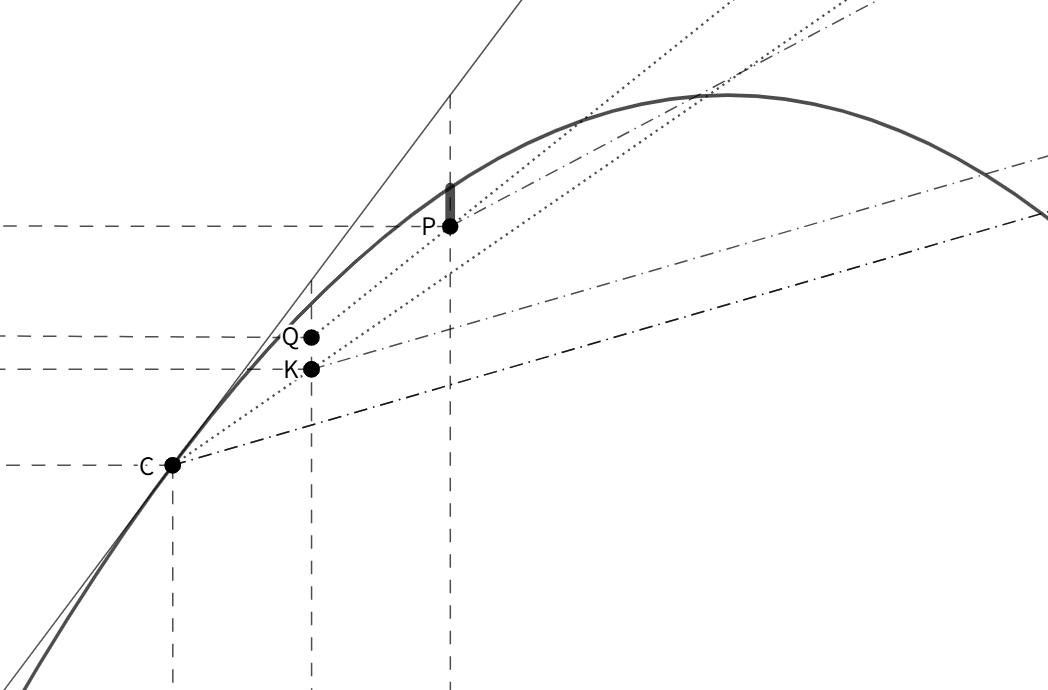
\includegraphics[width=0.6\textwidth]{figure/Exercise13-7.png}
    \caption{TR-BDF2 方法的几何图形}
    \label{fig:Exercise13-7}
\end{figure}

\section*{Exercise 13.11}

\par 对于显式中点方法， 其迭代公式为
\begin{equation}
    \left\{
        \begin{aligned}
            &y_1 = f(U^n,t_n) \\
            &y_2 = f\Big(U^n+\frac{k}{2}f(U^n,t_n),t_{n}+\frac{k}{2}\Big) \\
            &U^{n+1} = U^n + ky_2 \\
        \end{aligned}
    \right.
\end{equation}
\par 先对 $y_2$ 进行 Taylor 展开
\begin{equation}
    \begin{aligned}
        y_2 &= f\Big(U^n+\frac{k}{2}f(U^n,t_n),t_{n}+\frac{k}{2}\Big) \\
        &= f 
        + \left(\frac{k}{2}f_t + \frac{kf}{2} f_u\right)
        + \left(
            \frac{k^2}{8} f_{tt} + \frac{k^2f}{4} f_{ut} + \frac{(kf)^2}{8}  f_{uu}
        \right) + O(k^3)
    \end{aligned}
\end{equation} 
\par 其一步误差为
\begin{equation}
    \begin{aligned}
        \mathcal{L}u(t_n)
        =&\ u(t_{n+1}) - u(t_n) - ky_2 \\
        =&\ \left[
            u(t_n) +ku'(t_n)+\frac{k^2}{2}u''(t_n)+\frac{k^3}{6}u'''(t_n) - u(t_n) + O(k^4)
        \right]  \\
        &- k\left[
            f 
            + \left(\frac{k}{2}f_t + \frac{kf}{2} f_u\right)
            + \left(
                \frac{k^2}{8} f_{tt} + \frac{k^2f}{4} f_{ut} + \frac{(kf)^2}{8}  f_{uu}
            \right) + O(k^3)
        \right]\\
        =&\ \left[
            kf+\frac{k^2}{2}\left(ff_u+f_t\right)+\frac{k^3}{6}\left(
                f^2_uf+f_uf_t+f^2f_{uu}+2ff_{ut}+f_{tt}
            \right) + O(k^4)
        \right]  \\
        &- k\left[
            f 
            + \left(\frac{k}{2}f_t + \frac{kf}{2} f_u\right)
            + \left(
                \frac{k^2}{8} f_{tt} + \frac{k^2f}{4} f_{ut} + \frac{(kf)^2}{8}  f_{uu}
            \right) + O(k^3)
        \right]\\
        =&\ \frac{1}{24}k^3\left(
            4f^2_uf+4f_uf_t+f^2f_{uu}-2ff_{ut}+f_{tt}
        \right) + O(k^4)
    \end{aligned}
\end{equation}
\par 因此该方法有二阶精度。

\section*{Exercise 13.20}

\par TR-BDF2 方法的迭代公式为
\begin{equation}
    \left\{
        \begin{aligned}
            &\mathbf{U}^* = \mathbf{U}^n + \frac{k}{4}\left(
                \mathbf{f}(\mathbf{U}^n,t_n)+\mathbf{f}\left(\mathbf{U}^*,t_{n}+\frac{k}{2}\right)
            \right) \\
            &\mathbf{U}^{n+1} = \frac{1}{3}\left(
                4\mathbf{U}^* - \mathbf{U}^n + k \mathbf{f}(\mathbf{U}^{n+1},t_{n+1})
            \right)
        \end{aligned}
    \right.
\end{equation}
\par 代入测试函数 $u'(t)=\lambda u$ 得到
\begin{equation}
    \left\{
        \begin{aligned}
            &U^* = U^n + \frac{k}{4}\left(
                \lambda U^n+\lambda U^*
            \right) \\
            &U^{n+1} = \frac{1}{3}\left(
                4U^* - U^n + k \lambda U^{n+1}
            \right)
        \end{aligned}
    \right.
\end{equation}
\par 将 $U^*$ 用 $U^n$ 表示出来得到
\begin{equation}
    U^* = \frac{1+\frac{1}{4}k\lambda}{1-\frac{1}{4}k\lambda}U^n
\end{equation}
\par 代入 $U^{n+1}$ 的迭代公式中得到
\begin{equation}
    \begin{gathered}
        U^{n+1} = \frac{1}{3}\left(
        4\cdot\frac{1+\frac{1}{4}k\lambda}{1-\frac{1}{4}k\lambda}U^n - U^n + k \lambda U^{n+1}
            \right) \\
        U^{n+1} = \frac{1}{3}\left(
        \frac{3+\frac{5}{4}k\lambda}{1-\frac{1}{4}k\lambda}U^n + k \lambda U^{n+1}
            \right) \\
        U^{n+1} = \frac{1+\frac{5}{12}k\lambda}{1-\frac{7}{12}k\lambda+\frac{1}{12}
        (k\lambda)^2}U^n
    \end{gathered}
\end{equation}
\par 令 $z=k\lambda$ 则得到 TR-BDF2 方法的稳定函数 $R(z)$。
接下来可以通过 Taylor 展开来分析 $R(z)$ 的阶数。
\begin{equation}
    \begin{aligned}
        R(z)-e^z &= \frac{1+\frac{5}{12}z}{1-\frac{7}{12}z+\frac{1}{12}z^2}-e^z \\
        &= \left(
            1+\frac{5}{12}z
        \right)\left[
            1+\left(\frac{7}{12}z-\frac{1}{12}z^2\right)
            +\cdots+\left(\frac{7}{12}z-\frac{1}{12}z^2\right)^3+O(z^4)
        \right]-e^z \\
        &= \left(
            1+\frac{5}{12}z
        \right)\left[
            1+\left(\frac{7}{12}z-\frac{1}{12}z^2\right)
            +\left(\frac{49}{144}z^2-\frac{7}{72}z^3\right)
            +\left(\frac{343}{1728}z^3\right)+O(z^4)
        \right]-e^z \\
        &= \left(
            1+\frac{5}{12}z
        \right)\left[
            1+\frac{7}{12}z+\frac{37}{144}z^2
            +\frac{175}{1728}z^3+O(z^4)
        \right]-e^z \\
        &= \left(
            1+z+\frac{1}{2}z^2+\frac{5}{24}z^3
            +O(z^4)
        \right)-e^z \\
        &= \frac{1}{24}z^3
            +O(z^4)
    \end{aligned}
\end{equation}

\section*{Exercise 13.25}

\par 如图 \ref{fig:Exercise13-25} 所示，当 $\lambda_0=-10^6$ 时，
Backward Euler 方法的数值解非常接近于精确解，而 Trapezoidal 方法的数值解则发生了震荡。
这是因为 Trapezoidal 方法的稳定函数 $R(z)$ 的模在 $z=-10^6$ 
时非常接近于 $-1$，也就是$|R(z)|\rightarrow 1$，在稳定域的边界上，
可能由于数值误差的存在导致数值解发生震荡。


\begin{figure}[htbp]
    \centering
    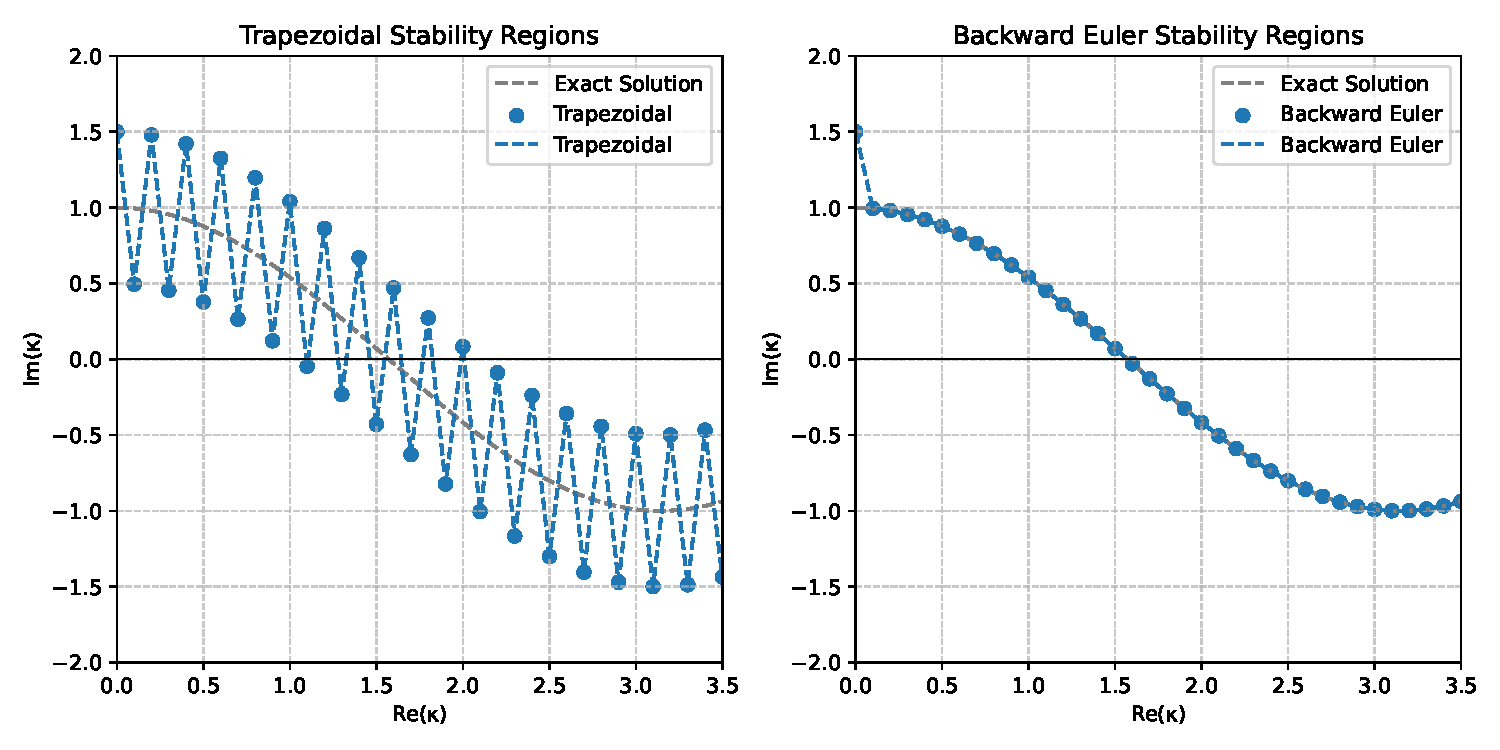
\includegraphics[width=0.8\textwidth]{figure/Exercise13-25.pdf}
    \caption{Trapezoidal 方法和 Backward Euler 方法的数值解}
    \label{fig:Exercise13-25}
\end{figure}


% ===============================================

\printbibliography

\end{document}